
En esta seccion mostramos las reglas de los juegos y como se pagan las apuestas.
No modelamos entre otras cosas, el casino, la historia, etc. las distintas mesas.
Tampoco la cola de tiradore ni tenemos en cuenta los clientes vips, para ver ese
comportamiento de se debe obviar la guarda que chequea si el saldo le alcanza para apostar.

Esencialmente cada máquina muestra parte del comportamiento del caso de uso:
\begin{itemize}
 \item Jugando tragamonedas : FSM Tragamonedas
 \item Jugando Craps: FSM Craps
\end{itemize}

Observaciones sobre las m'aquinas:
dadas las limitaciones del software que utilizamos para dibujarlas y por razones 
de hacerlas más legibles cambiamos levemente la convensi'on, a saber:
\begin{itemize}
 \item El estado inicial lleva la etiqueta ``inicial''
\item La guarda se pone al lado de la transici'on entre corchetes
\item el efecto lleva una ``/''
\end{itemize}

Otra libertad que tomamos en pos de la legibilidad fue extender un poco 
la idea de reescritura con ``...'', en las m'aquinas \textit{FSM apuestas de sitio a ganar} y \textit{FSM apuestas de sitio a perder i} en las transiciones tanto de agregar fichas, como de quitar, para no repetir trancisiones que agregaran ilegibilidad a la m'aquina, entonces:
donde dice: `` 5, seis, 8, nueve'', deben agrearse las trancisiones que reperesenten esas, agregardos, modificaciones de 
fichas o pagos.



\subsection{Variables}

\begin{itemize}
\item dados [ 2 ... 12]
\item valor punto [2 ... 12]
\item apuesta venir i [0 ... MAX]
\item VF tupla de 1 a M valores, contienen el valor de cada una de las M fichas
\item saldo i [0... MAX]
\item puntaje NO venir [0 ... 12]
\item Apuesta de campo [0 ...  MAX]
\item MA es la matriz de apuestas cada posisción lleva la cantidad de fichas, cada columna es la ficha, cada fila el numero por cual apost'o.
\item fichas apostadas i = [1..3]
\item valor ficha i

\end{itemize}



	\subsubsection{FSM Craps}




FSM Craps es la composici'on en paralelo de : 
FSM Apuesta de Campo i (fig. \ref{fig:apDeCampo}) $|$ 
FSM Apuesta de Sitio a Ganar i (fig. \ref{fig:apSitioAGanar}) $|$
FSM Apuesta de Sitio a Perder i (fig. \ref{fig:apDeSitioAPerder}) $|$
FSM Apuesta Linea de No Pase i (fig. \ref{fig:FSM_ApuestaLineaDeNoPase}) $|$
FSM Apuesta Linea de Pase i (fig. \ref{fig:FSM_ApuestaLineaDePase}) $|$
FSM Apuesta NoVenir i (fig. \ref{fig:FSM_ApuestaNoVenir})$|$
FSM Apuesta Venir i (fig. \ref{fig:FSM_ApuestaVenir}) $|$
FSM Dados i (fig. \ref{fig:FSM_Dados}) $|$


        \begin{figure}[p!hbt]
		\centering
		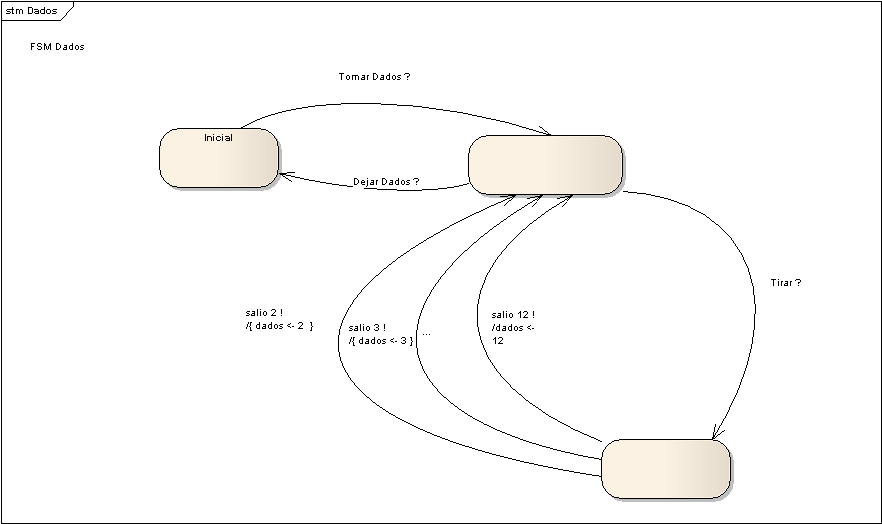
\includegraphics[angle=0, width=0.8\textwidth]{../img/FSM_Dados.png}
		\caption{FSM Dados }
		\label{fig:FSM_Dados}
	\end{figure}

        \begin{figure}[p!hbt]
		\centering
		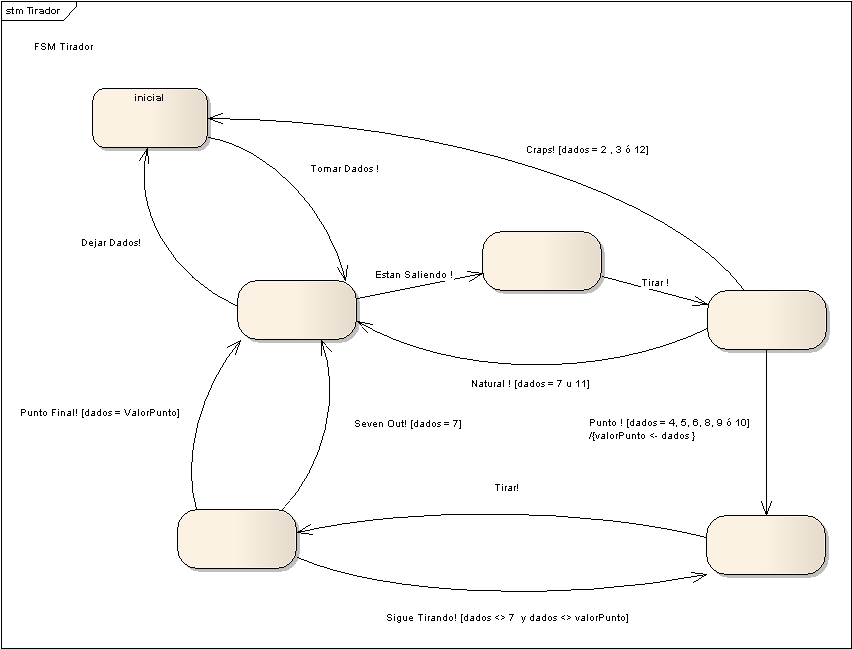
\includegraphics[angle=0, width=0.8\textwidth ]{../img/FSM_Tirador.png}
		\caption{FSM Tirador }
		\label{fig:fsmtirador}
	\end{figure}


        \begin{figure}[p!hbt]
		\centering
		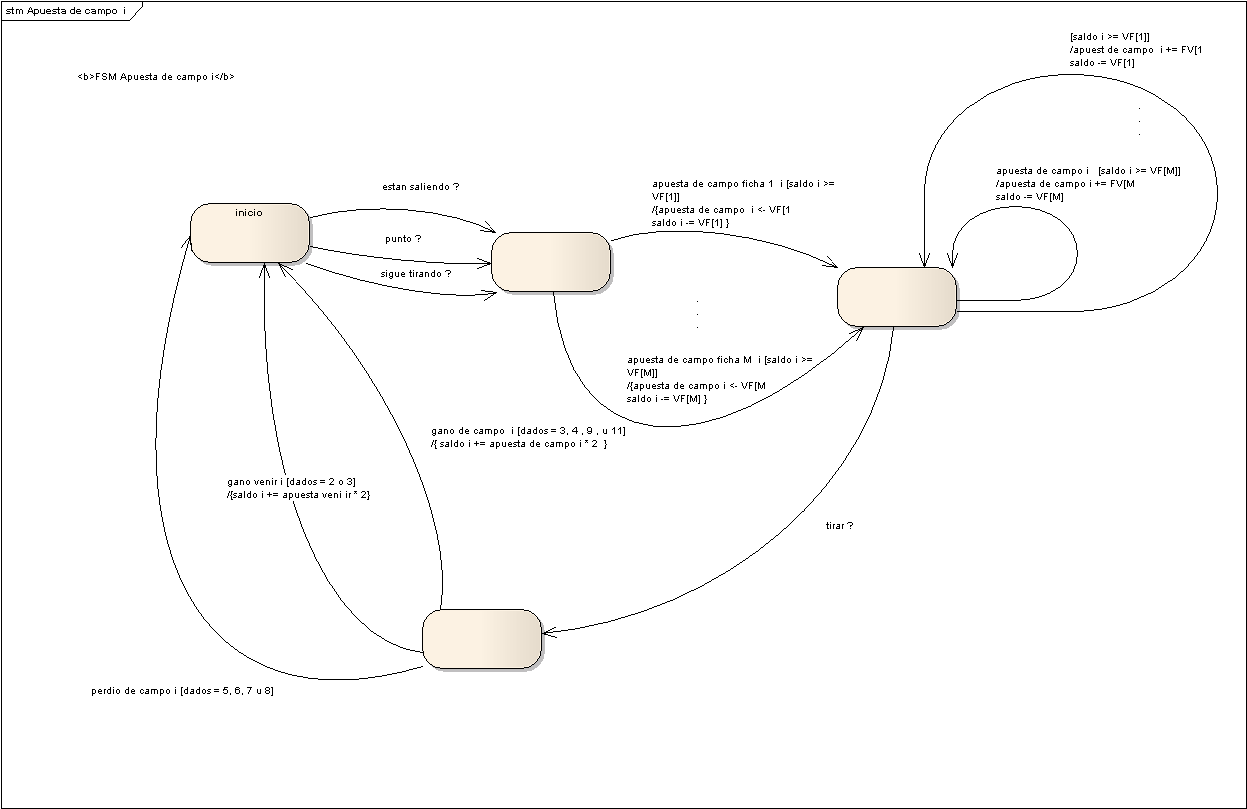
\includegraphics[angle=90, width=0.9\textwidth]{../img/FSM_ApuestaDeCampo}
		\caption{FSM Apuestas de Campo i }
		\label{fig:apDeCampo}
	\end{figure}



        \begin{figure}[p!hbt]
		\centering
		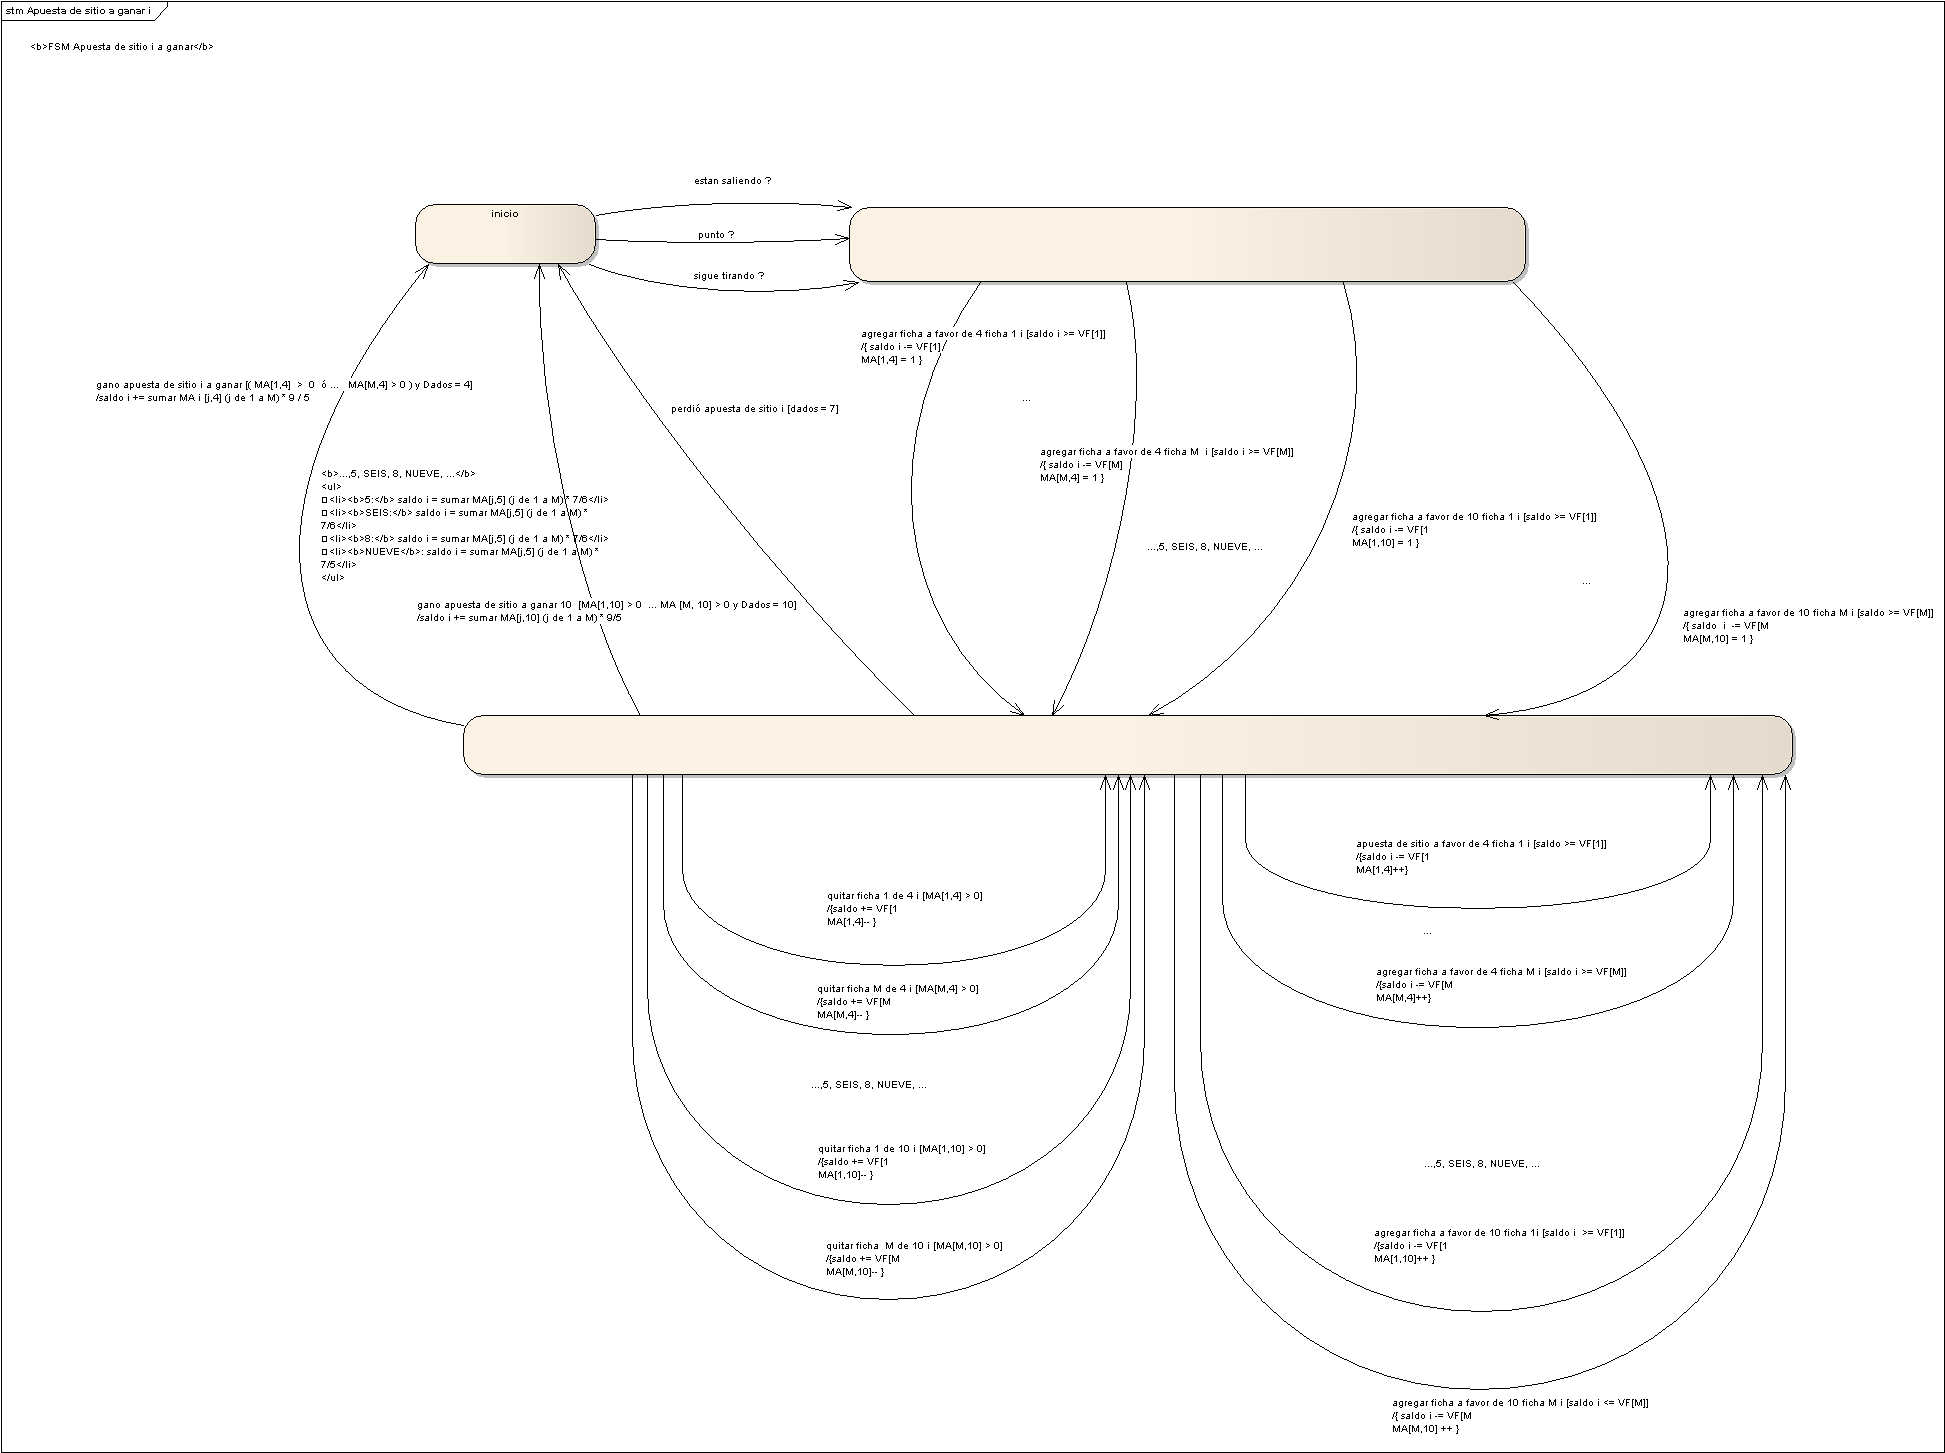
\includegraphics[angle=90, width=0.9\textwidth]{../img/FSM_ApuestaDeSitioAGanar.png}
		\caption{FSM Apuesta de Sitio a Ganar i}
		\label{fig:apSitioAGanar}
	\end{figure}


        \begin{figure}[p!hbt]
		\centering
		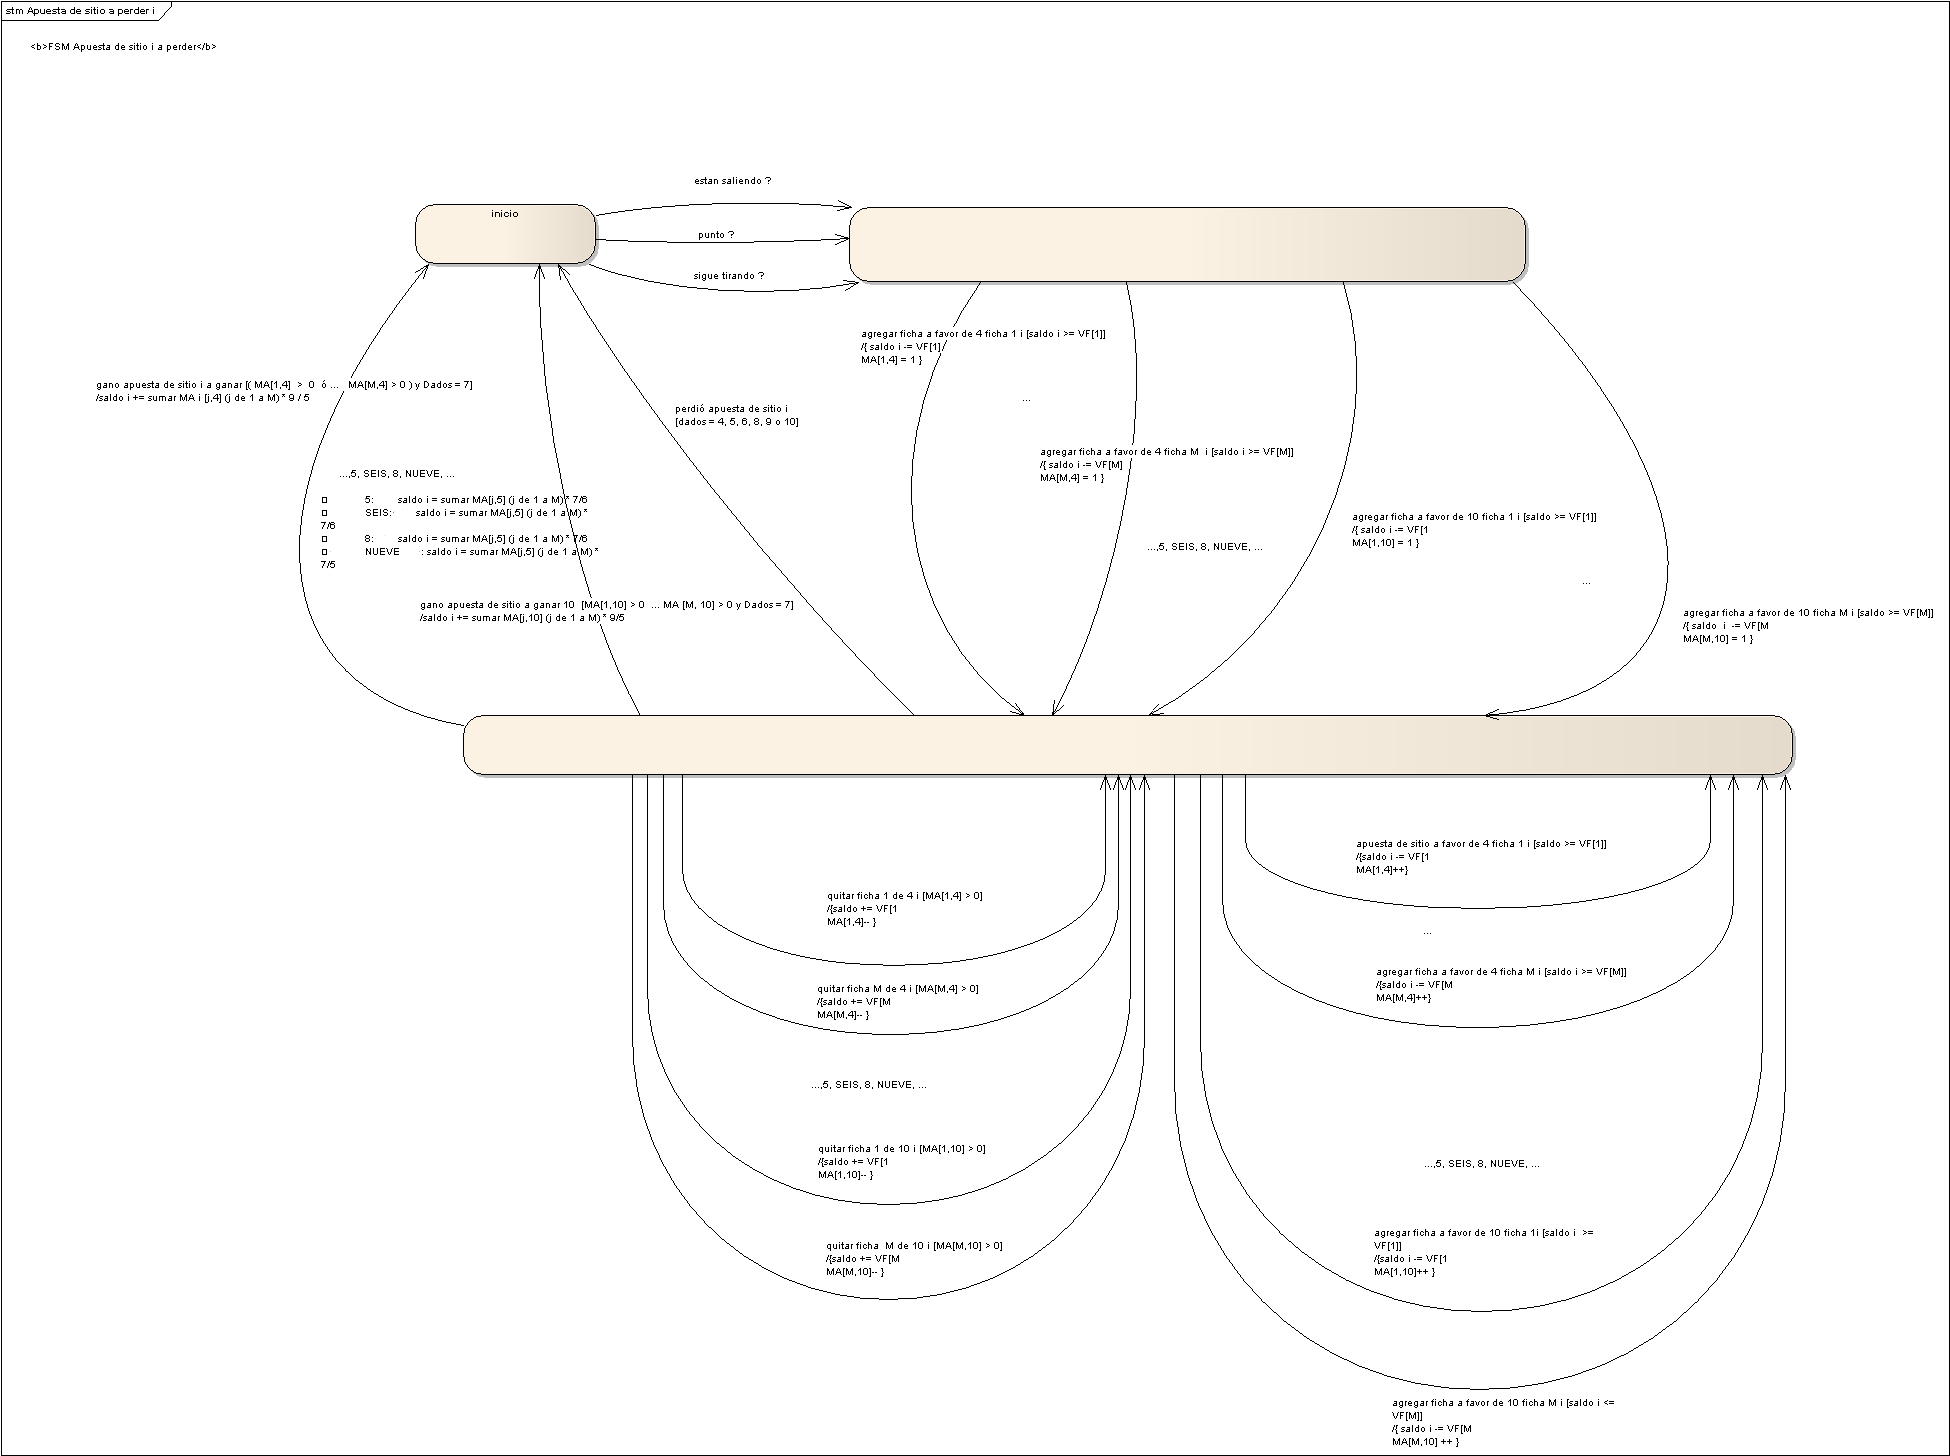
\includegraphics[angle=90, width=0.9\textwidth]{../img/FSM_ApuestaDeSitioAPerder.png}
		\caption{FSM Apuesta de sitio a perder i }
		\label{fig:apDeSitioAPerder}
	\end{figure}

        \begin{figure}[p!hbt]
		\centering
		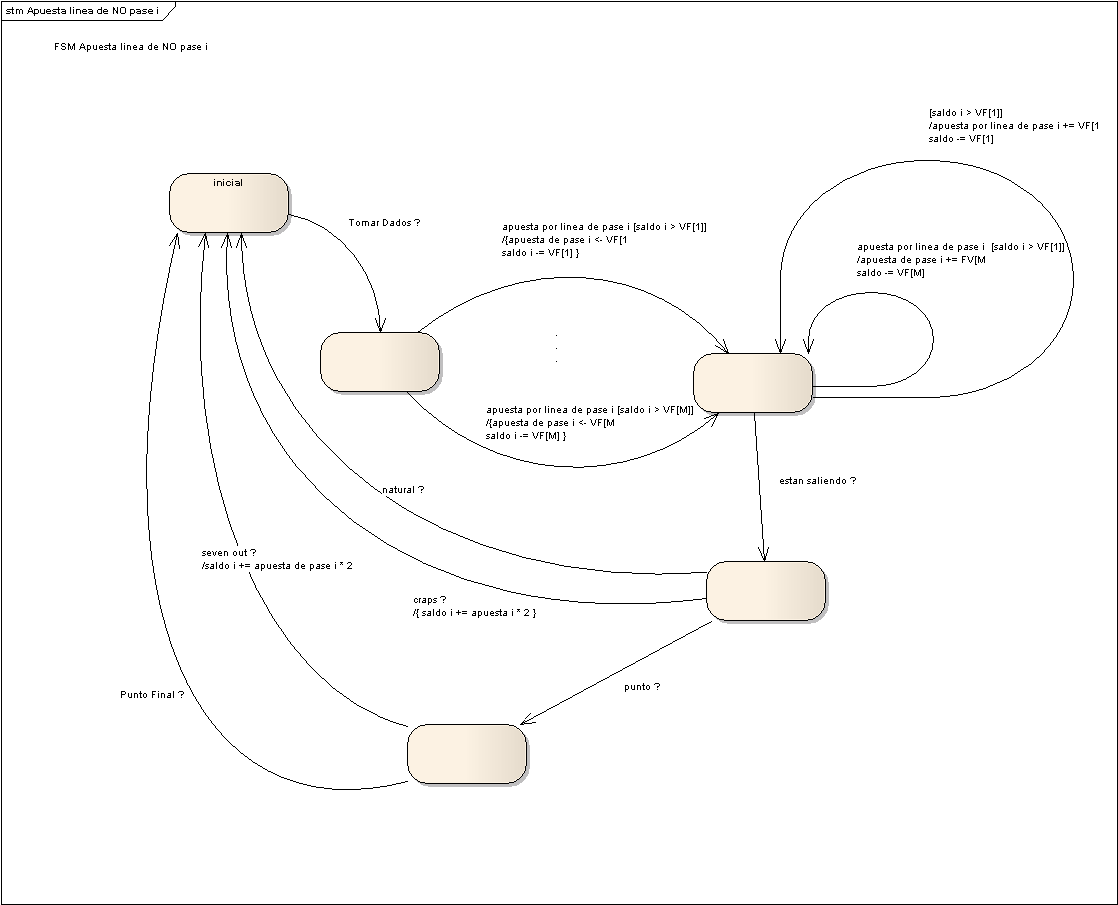
\includegraphics[angle=90, width=0.9\textwidth]{../img/FSM_ApuestaLineaDeNoPase.png}
		\caption{FSM Apuesta de linea de No pase i }
		\label{fig:FSM_ApuestaLineaDeNoPase}
	\end{figure}

        \begin{figure}[p!hbt]
		\centering
		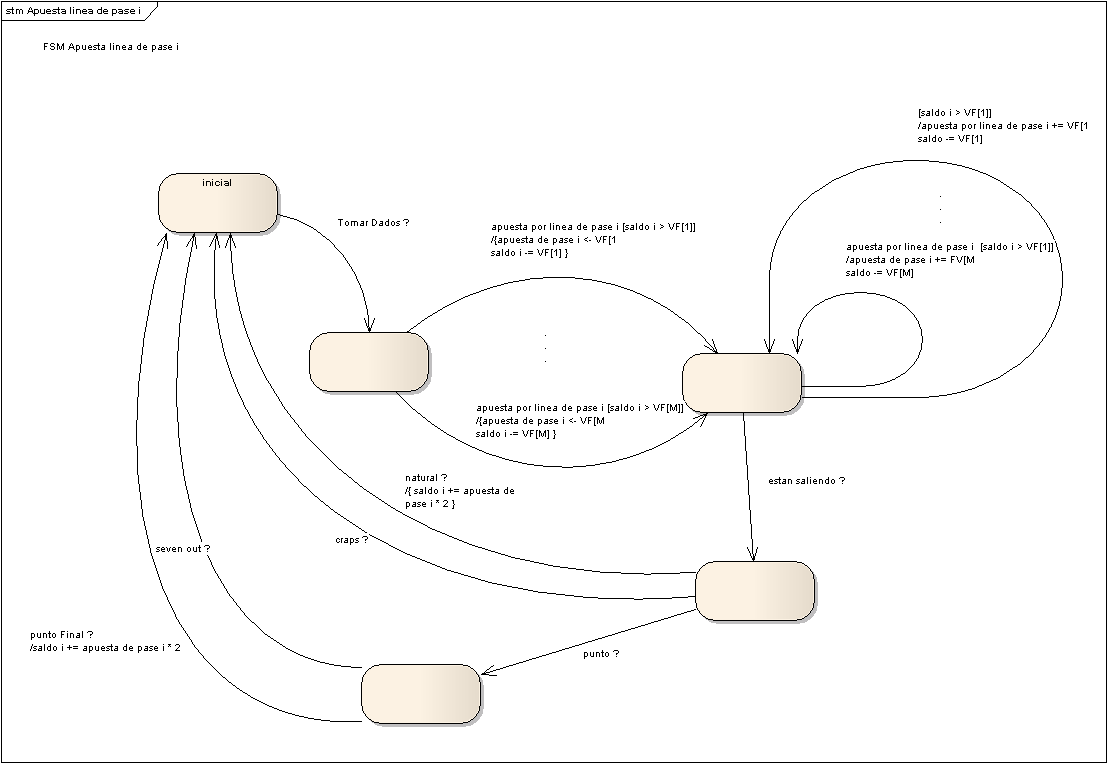
\includegraphics[angle=90, width=0.9\textwidth]{../img/FSM_ApuestaLineaDePase.png}
		\caption{FSM Apuesta de linea de pase i }
		\label{fig:FSM_ApuestaLineaDePase}
	\end{figure}

        \begin{figure}[p!hbt]
		\centering
		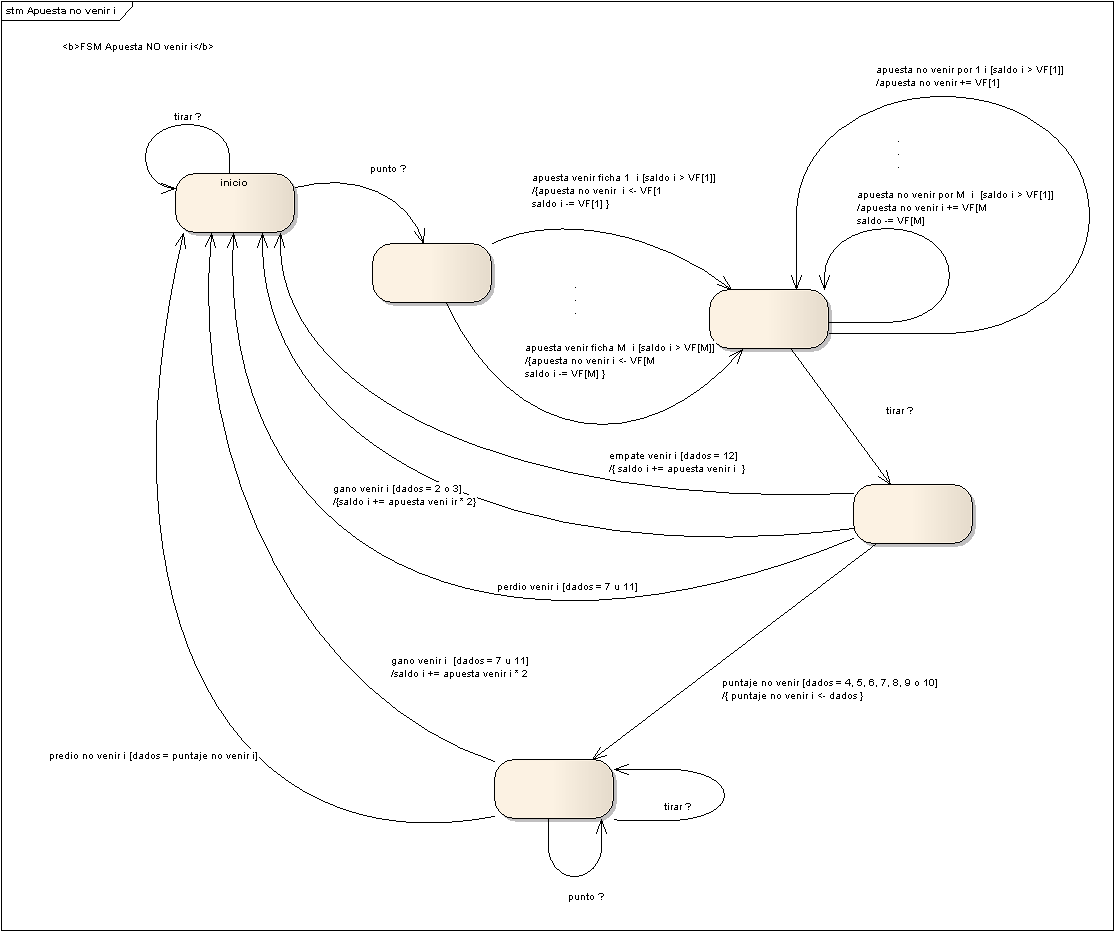
\includegraphics[angle=90, width=0.9\textwidth]{../img/FSM_ApuestaNoVenir.png}
		\caption{FSM Apuesta No Venir i }
		\label{fig:FSM_ApuestaNoVenir}
	\end{figure}

        \begin{figure}[p!hbt]
		\centering
		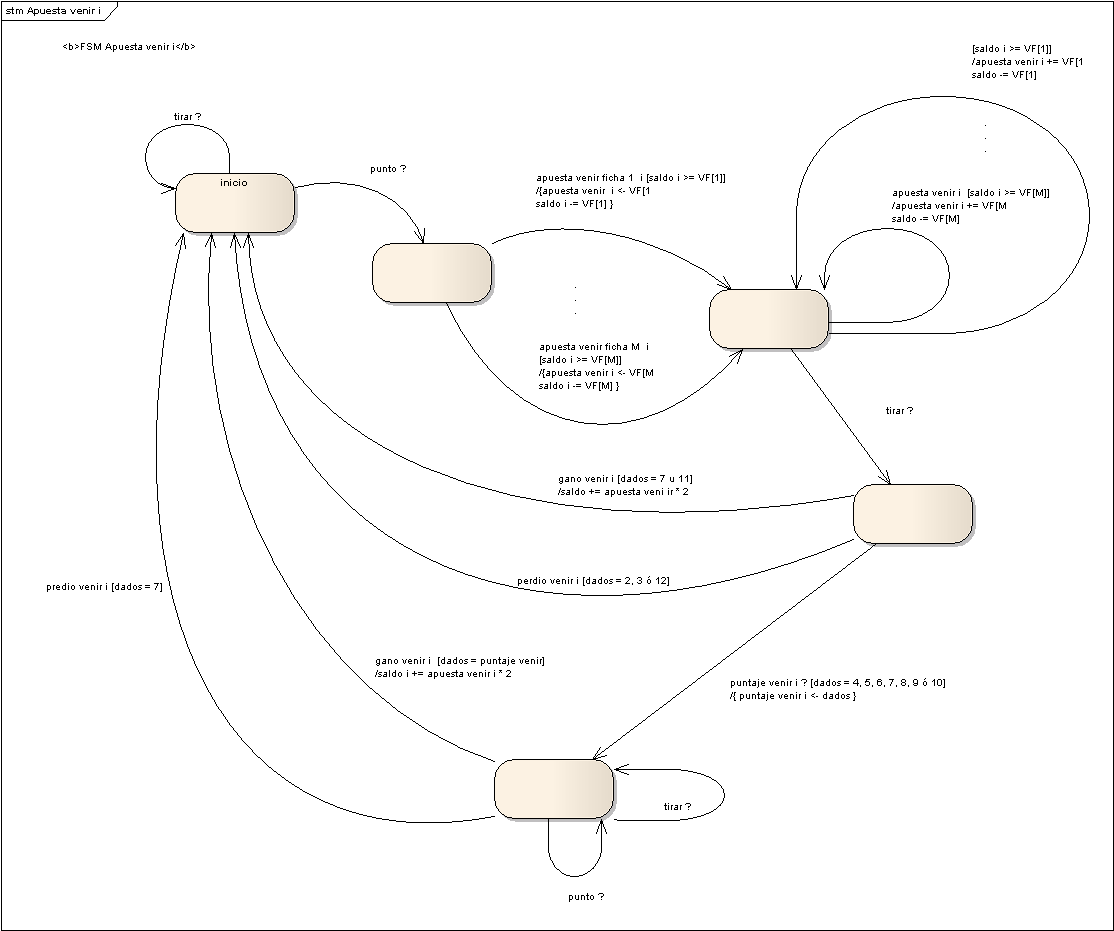
\includegraphics[angle=90, width=0.9\textwidth]{../img/FSM_ApuestaVenir.png}
		\caption{FSM Apuesta Venir i }
		\label{fig:FSM_ApuestaVenir}
	\end{figure}



\subsubsection{FSM Tragamonedas}

FSM Tragamonetas es la composici'on en paralelo de : 

FSM Juego Tragamonedas i (fig. \ref{fig: FSMtraga}) $|$
FSM Jugador Tragamonedas i (fig. \ref{fig:FSMjugadorTraga} 


        \begin{figure}[p!hbt]
		\centering
		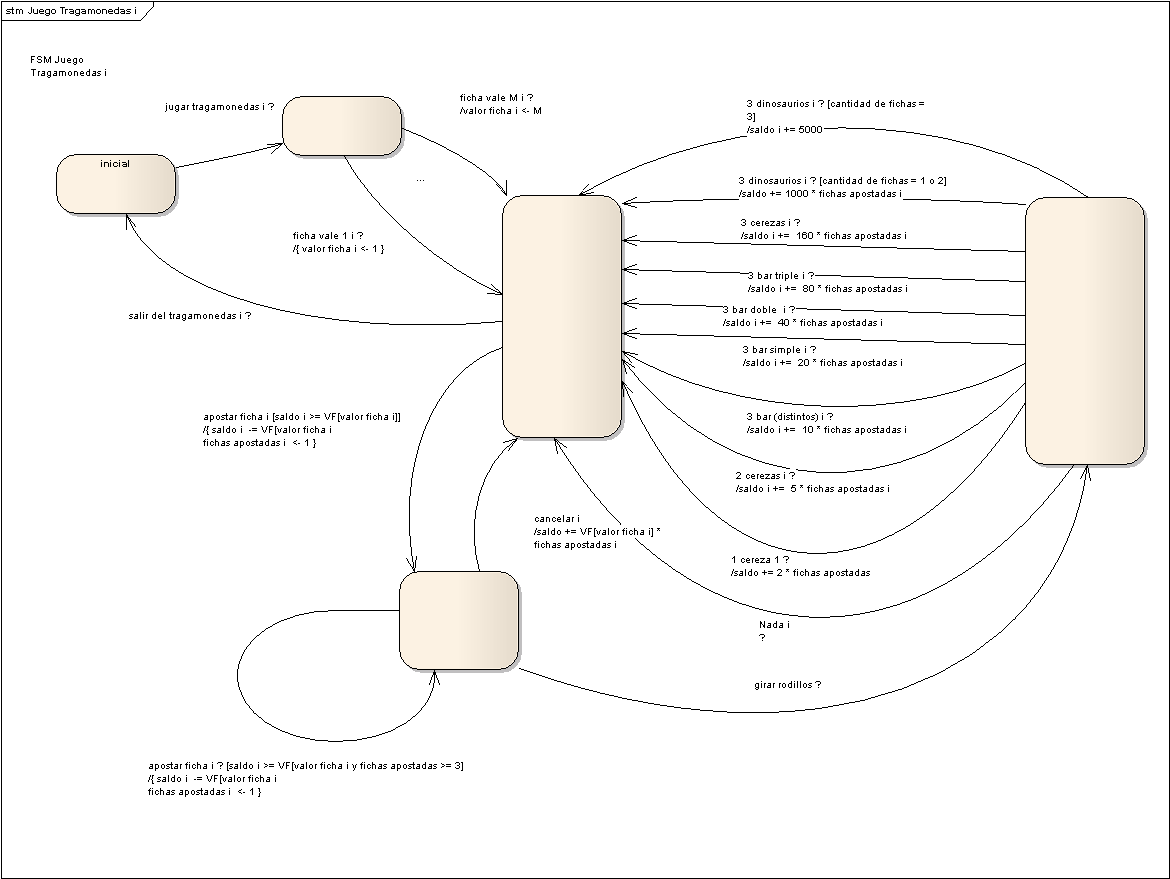
\includegraphics[angle=90, width=0.9\textwidth]{../img/FSM_JuegoTragamonedas.png}
		\caption{FSM Juego Tragamonedas }
		\label{fig: FSMtraga}
	\end{figure}

        \begin{figure}[p!hbt]
		\centering
		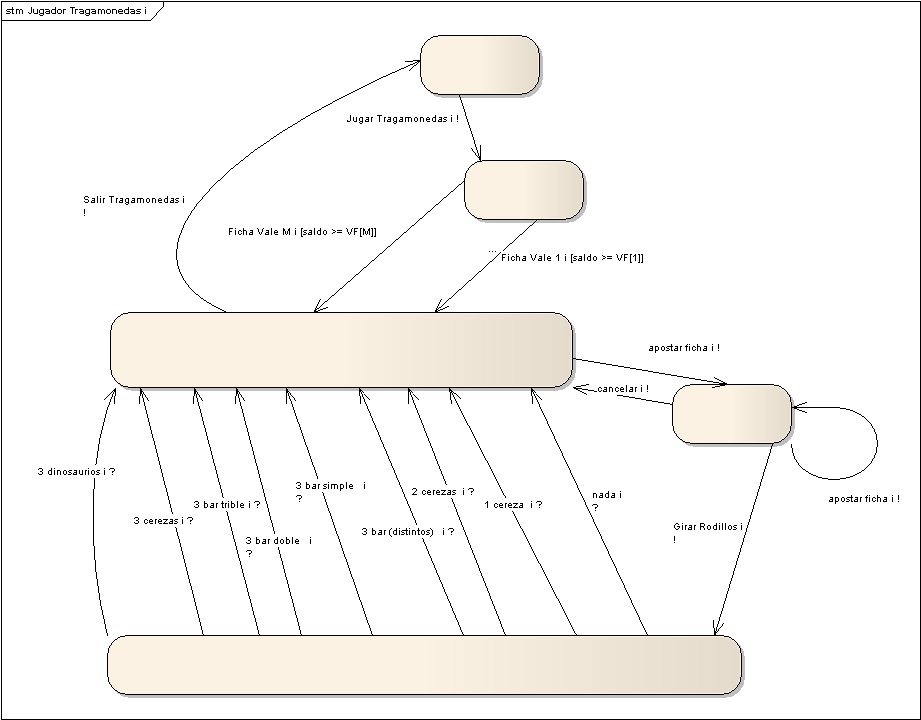
\includegraphics[angle=90, width=0.9\textwidth]{../img/FSM_JugadorTragamonedas.png}
		\caption{FSM Jugador Tragamonedas }
		\label{fig:FSMjugadorTraga}
	\end{figure}


